%!TEX root = ../main.tex

\chapter{Literature Review}\label{cha:literature}

Many extensive literature reviews and surveys have been written on the subject of deep learning.
In 1987, Lippmann reviewed 6 of the most influential Neural Networks of the era \cite{Lippmann_1987}.
More recently, an extensive Survey on Deep Learning in Medical Image Analysis was published \cite{Litjens_Kooi_Bejnordi_Setio_Ciompi_Ghafoorian_van_der_Laak_van_Ginneken_Sanchez_2017}.
In this, the use of deep learning for image classification, object detection and segmentation are all reviewed.
Also overviews of anatomical areas are provided, including neuro, retinal, pulmonary, digital pathology, breast, cardiac, abdominal and musculoskeletal.

\section{Deep Learning}\label{sec:deep_learning_lit}

\subsection{Training Deep Neural Networks}\label{subsec:training}
Due to the size of deep neural networks, and the non-convexity of the parameters, finding good optima has always been a challenge.
Stochastic gradient descent (SGD) has remained a popular strategy for researchers since the 80's although many optimisation algorithms are now used.
These include Adam \cite{Kingma_Ba_2014}, ADADELTA \cite{Zeiler_2012} and AdaGrad \cite{Duchi_Hazan_Singer_2011}.
For all of the optimisers mentioned, one of the main issues during training is choosing an appropriate learning rate.

It has been suggested by Dauphin et al. in \cite{Dauphin_de_Vries_Bengio_2015} that saddle points cause issues during training, not poor local optima.
However, in The Deep Learning Book \cite{Goodfellow-et-al-2016}, Goodfellow et al. prove that although learning is slow around saddle points due to the flatness, gradient based optimisation algorithms are still able to escape.

One possible solution is to use cyclical learning rates instead of a fixed learning rate that decreases over time.
A cycle has a fixed length and the learning rate varies between two sensible boundary values during that cycle.
This helps because if the optimisation gets stuck on a saddle plateau, increasing the learning rate will traverse the plateau quickly.

In Figure \ref{fig:triangular_cyclical_learning_rate} two methods for cyclical learning rates are shown.
Leslie N. Smith propesed these in \cite{Smith_2015}.
On the left plot min and max learning rate are kept the same, wheras on the right the difference is cut in half after each cycle.


\begin{figure}[hbtp!]
    \centering
    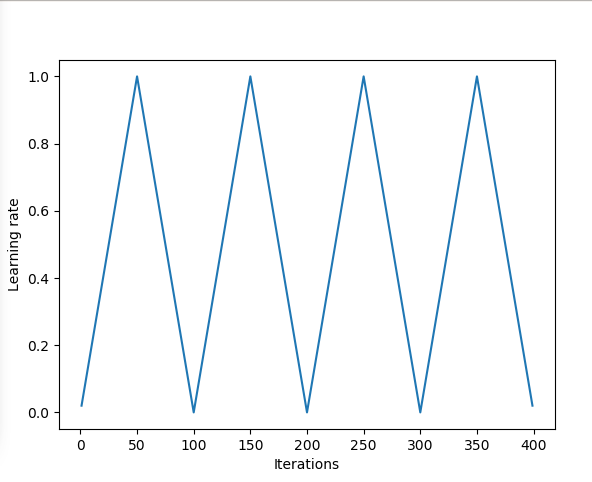
\includegraphics[width=0.45\textwidth]{./img/triangular.png}
    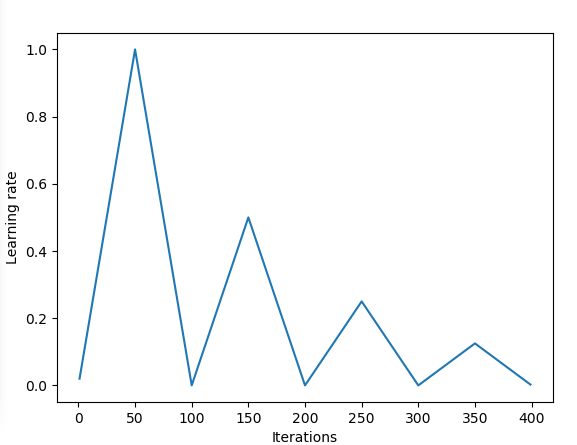
\includegraphics[width=0.45\textwidth]{./img/triangular2.png}
    \caption{Triangular and Triangular2 by Leslie N. Smith \cite{Smith_2015}.}
    \label{fig:triangular_cyclical_learning_rate}
\end{figure}

An alternative was suggested by Loshchilov and Hutter in \cite{Loshchilov_Hutter_2016} called Cosine Annealing.
In this, the learning rate starts at its maximum and decreases to its minimum following the cosine function.
Once the minimum is reached the learning resets to the maximum, there is no increasing phase.
The learning rate $\eta$ is given by:

\begin{equation}
    \eta = \eta_{min} + \frac{1}{2}(\eta_{max} - \eta_{min})(1 + \cos(\frac{T_{cur}}{T_i}\pi)
    \label{eq:cosine_annealing}
\end{equation}

Where $\eta_{min}$ and $\eta_{max}$ are the minimum and maximum learning rates respectively.
$T_{cur}$ is the number of iterations since the previous restart and $T_i$ is the number of iterations within each run.

The authors also suggest making each cycle longer than the last.
This is acheived by increasing $T_i$ after each cycle by a constant factor $T_{mult}$.
Figure \ref{fig:cosine_annealing} shows Cosine Annealing with $T_{mult}=1$ on the left and $T_{mult}=2$ on the right.
In the case of $T_{mult}=1$ this is completely equivalent to Equation \ref{eq:cosine_annealing}.

\begin{figure}[hbtp!]
    \centering
    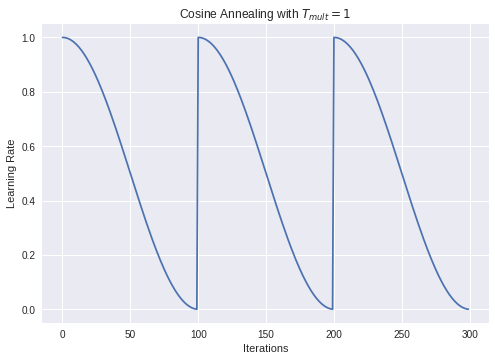
\includegraphics[width=0.45\textwidth]{./img/tmul1.png}
    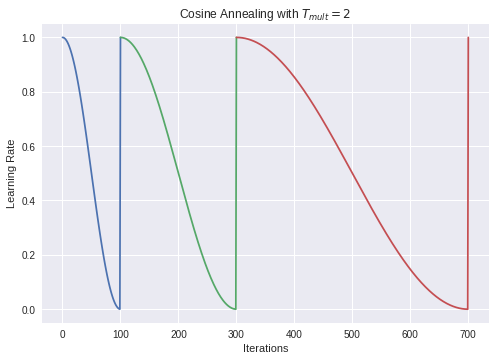
\includegraphics[width=0.45\textwidth]{./img/tmul2.png}
    \caption{Cosine Annealing with $T_{mult}=1$ and $T_{mult}=2$ by Loshchilov and Hutter \cite{Loshchilov_Hutter_2016}.}
    \label{fig:cosine_annealing}
\end{figure}

It is well known that the number of local minima increases exponentially with the number of parameters \cite{Kawaguchi_2016}.
Given that modern neural networks may contain millions of parameters, it is clear that identical architectures with different initialisation will converge to different solutions.
Often local minima have very similar error rates, however the corresponding neural networks will make different mistakes.

This can be exploited using ensembling methods similar to those described by \cite{Caruana_Niculescu-Mizil_Crew_Ksikes_2004}.
In \cite{Huang_Li_Pleiss_Liu_Hopcroft_Weinberger_2017} an ensembling method for Deep Learning is described which they call Snapshot Ensembling.
It extends the work of Loshchilov and Hutter \cite{Loshchilov_Hutter_2016} yet requires no additional training time.
This was achieved by saving the model weights at the end of each learning rate cycle ie. taking a snapshot.
Each time the learning rate is reset the neural net converges to a new local optima producing a substantially different model.
In the right hand side of Figure \ref{fig:cosine_annealing}, each coloured sections corresponds to the model converging to a different local minima.
The saved models can then be used as an ensemble at prediction time.


\subsection{Recent Developments}\label{subsec:recent_improvements}

In this section, an overview of some more recent developments will be given.
First, an extension of learning rate cycling and ensemble methods will be discussed.
Finally, Hinton's breakthrough regarding Capsule Networks will also be presented.

In \cite{Keskar_Mudigere_Nocedal_Smelyanskiy_Tang_2016} it is suggested that convergence to sharp minima leads to poor generalisation for deep learning.
The motivation for this suggestion is that the training loss surface and test loss surface will be similar but not exactly the same; one may be shifted when compared to the other.
For sharp minima, a point with low loss during training may produce large loss during testing due to this shift.
Whereas for a wide minima, the effect of this shift would be reduced.
This is shown in Figure \ref{fig:wide_optima} where a sharp and wide minima are compared.

\begin{figure}[hbtp!]
    \centering
    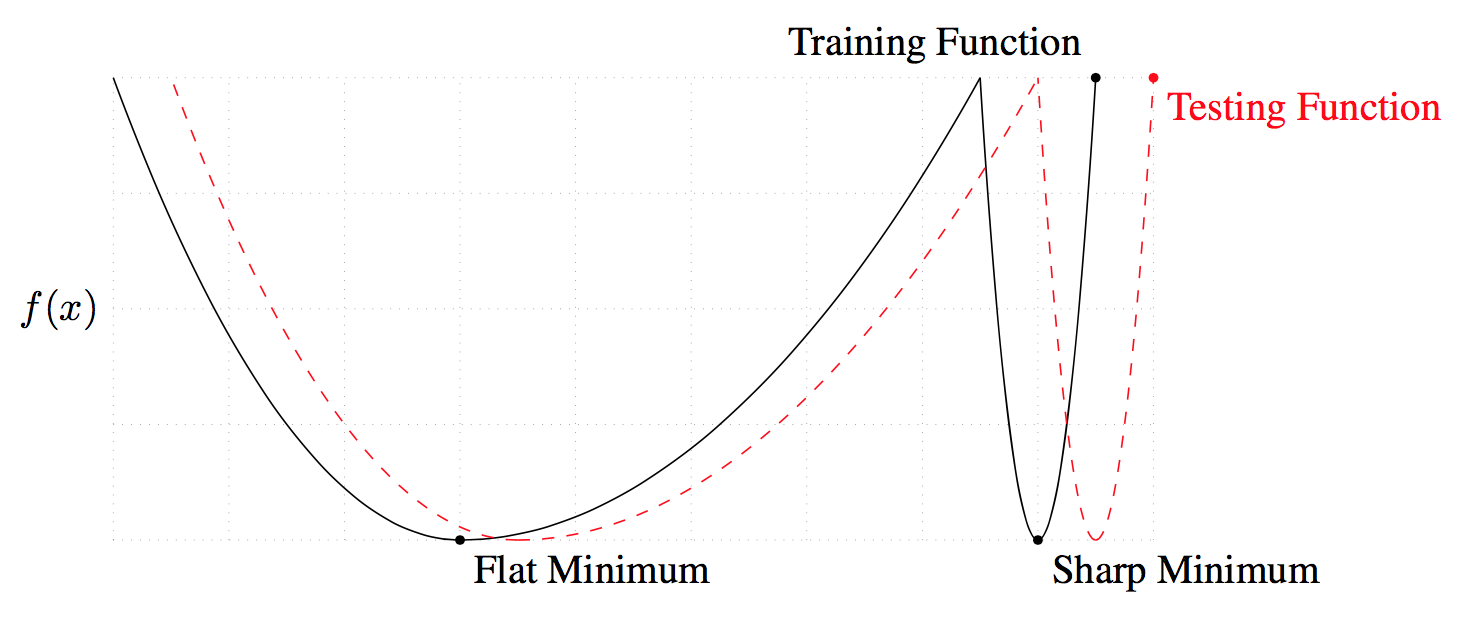
\includegraphics[width=\textwidth]{./img/Wide_optima.png}
    \caption{A Conceptual Sketch of Flat and Sharp Minima. The Y-axis indicates value of the loss function and the X-axis the variables (parameters) \cite{Keskar_Mudigere_Nocedal_Smelyanskiy_Tang_2016}}
    \label{fig:wide_optima}
\end{figure}

Numerical evidence is then given that supports this view and several attempts to address the problem are presented.
However, initial results suggest that whilst these strategies do lead to better generalisation, they still converge to sharp minima.
The next two methods are able to produce wide optima, and thus generalise very well at test time.

Fast Geometric Ensembling (FGE) is very similar to Snapshot Ensembling as described in Section \ref{sec:deep_learning_lit}.
The main differences are that it uses a piecewise linear cyclical learning rate (instead of cosine) and a much shorter cycle length.
A short cycle make seem intuitively wrong, because the saved models will not differ from each other much and therefore provide no benefit when taken as an ensemble.
However, in \cite{Garipov_Izmailov_Podoprikhin_Vetrov_Wilson_2018} it is shown that there exist connected paths of low loss between sufficiently different models and that it is possible to travel along those paths in small steps.
Thus the models encountered along the path will be different enough to allow ensembling them with good results.

Figure \ref{fig:FGE_shortest_path} demonstrates this concept on the cross-entropy loss surface of ResNet-164 on CIFAR-100.
The vertical axis changes between panels as we change planes.
The left plane shows three optima for independently trained networks.
These three optima are all isolated which agrees with standard intuition.
However, the middle and right panels show two different paths of near-constant loss, discovered by FGE training procedure.
The endpoints of the path correspond to two independently trained networks that coincide with the two lower optima in the left panel.
Notice that in each panel a direct linear path between each optima would incur high loss.

\begin{figure}[hbtp!]
    \centering
    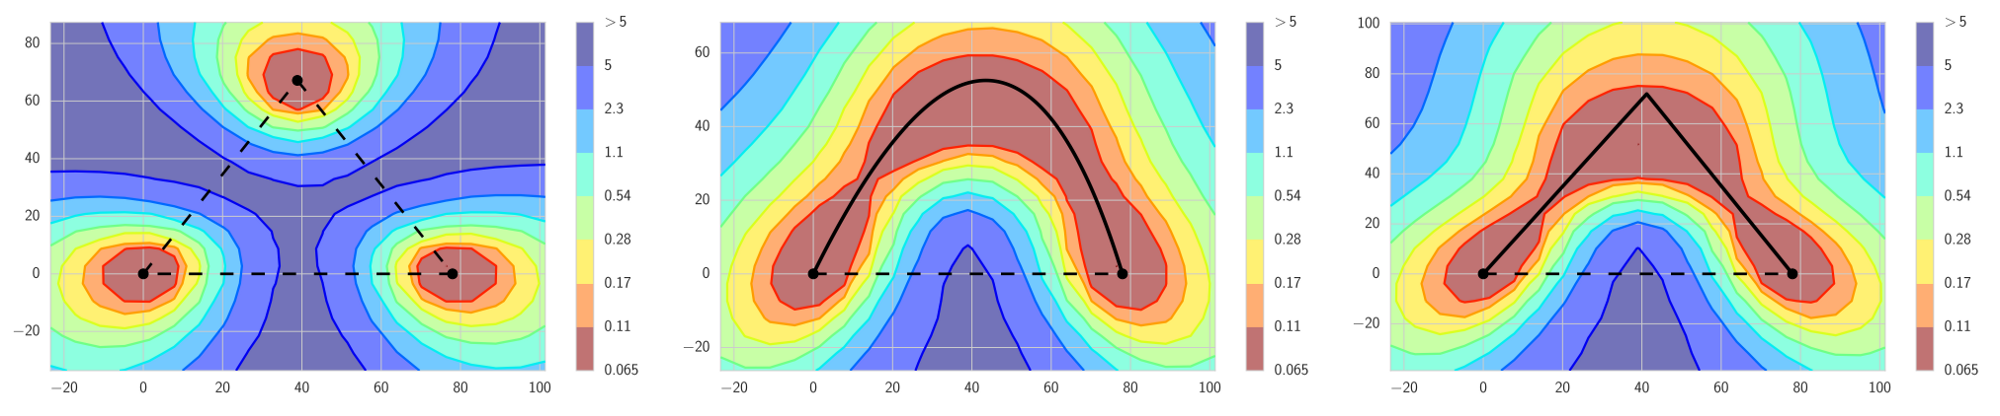
\includegraphics[width=\textwidth]{./img/FGE.png}
    \caption{The cross-entropy loss surface of a deep residual network (ResNet-164) on CIFAR-100, as a function of network weights in a two-dimensional subspace \cite{Garipov_Izmailov_Podoprikhin_Vetrov_Wilson_2018}.}
    \label{fig:FGE_shortest_path}
\end{figure}

FGE shows improvement on Snapshot Ensembling and due to the shorter learning rate cycle it is also faster to train.
However, to obtain the superior performance of FGE or Snapshort Ensembling many different models must be stored.
Also, predictions must be made by each model which are then averaged together, implying increased computations at test time.
In \cite{Izmailov_Podoprikhin_Garipov_Vetrov_Wilson_2018}, a training method is outlined that avoids this issue whilst maintaining comparable performance.

The methodologies discussed so far have been ensembles in model space; they use the predictions of several models to produce a final prediction.
In \cite{Izmailov_Podoprikhin_Garipov_Vetrov_Wilson_2018}, weights are averaged instead of model predictions.
This means that during training only two models need to be stored, and during testing only one model is used to make predictions.
The result 

\begin{figure}[hbtp!]
    \centering
    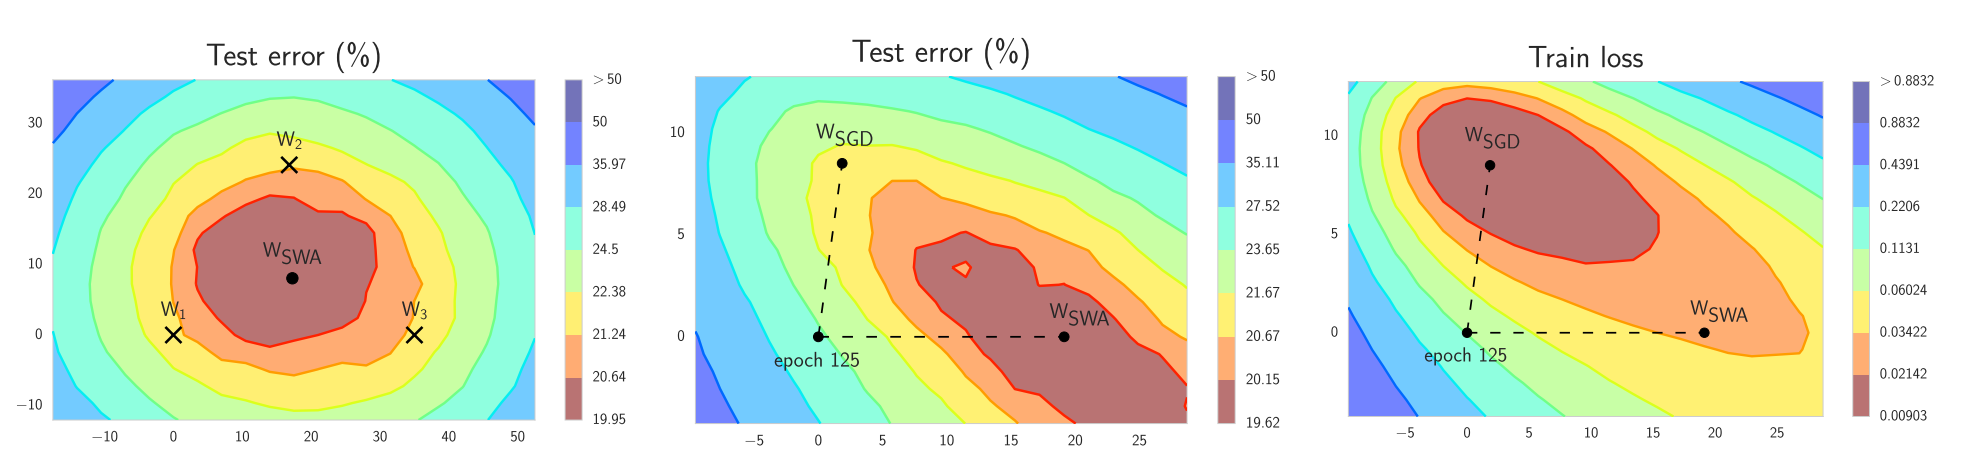
\includegraphics[width=\textwidth]{./img/SWA.png}
    \caption{\cite{Izmailov_Podoprikhin_Garipov_Vetrov_Wilson_2018}}
    \label{fig:SWA}
\end{figure}


% TODO SWA

We find that maintaining an average of the weights we encounter performs pretty well; it is better than snapshot and almost as good as FGE
This is much quicker and less computationally expensive because we don't have to carry around several different models. \cite{Izmailov_Podoprikhin_Garipov_Vetrov_Wilson_2018}


% TODO Capsule
In late 2017, Hinton outlined a method for training capsule based methods.
This is something he'd been thinking about for years.
It learns pose representations of objects. \cite{Hinton_Sabour_Frosst_2018, Sabour_Frosst_Hinton_2017}





\section{Deep Learning in Medicine}\label{deep_learning_medic_lit}
% TODO section on deep learning in medicine
U-Net \cite{Ronneberger_Fischer_Brox_2015}
3D U Net \cite{Cicek_Abdulkadir_Lienkamp_Brox_Ronneberger_2016}

Cancer metastases \cite{Liu_Gadepalli_Norouzi_Dahl_Kohlberger_Boyko_Venugopalan_Timofeev_Nelson_Corrado_et_al_2017}

Dermatologist level skin cancer \cite{Esteva_Kuprel_Novoa_Ko_Swetter_Blau_Thrun_2017}

TernausNet (pretrained weights as encoder part of unet) \cite{Iglovikov_Shvets_2018}
